% The compiler pipeline of chapter 1. Build with build-figure.sh.
\documentclass[tikz,border=6pt]{standalone}
\usepackage[T1]{fontenc}
\usepackage{helvet}
\renewcommand{\familydefault}{\sfdefault}
\usetikzlibrary{arrows.meta,decorations.pathreplacing}
% Light values. build-figure.sh maps them to the site theme's properties.
\definecolor{ink}{HTML}{0D1620}
\definecolor{muted}{HTML}{5A6874}
\definecolor{teal}{HTML}{00706B}
\begin{document}
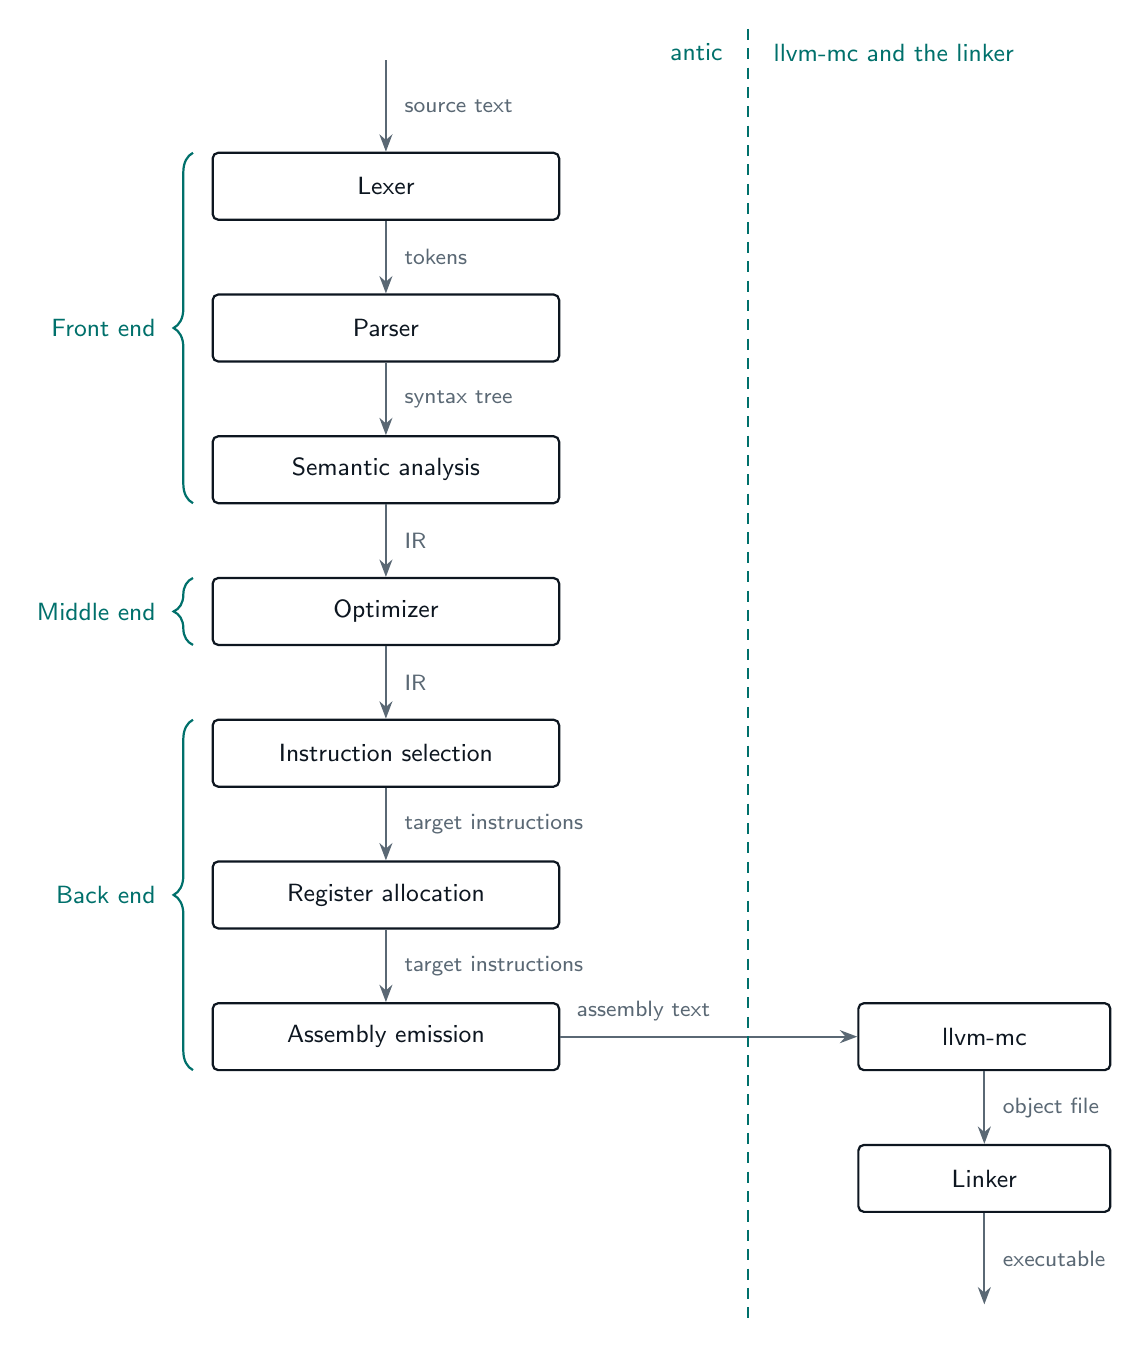
\begin{tikzpicture}[
  stage/.style={draw=ink, text=ink, line width=0.8pt, rounded corners=2pt,
    minimum width=4.4cm, minimum height=0.85cm, font=\small},
  tool/.style={stage, minimum width=3.2cm},
  flow/.style={draw=muted, line width=0.8pt, -{Stealth[length=2.2mm]}},
  artefact/.style={text=muted, font=\footnotesize},
  group/.style={draw=teal, line width=0.8pt,
    decorate, decoration={brace, amplitude=7pt}},
  grouplabel/.style={text=teal, font=\small, anchor=east},
]
\node[stage] (lex)    at (0,  0.0) {Lexer};
\node[stage] (parse)  at (0, -1.8) {Parser};
\node[stage] (sema)   at (0, -3.6) {Semantic analysis};
\node[stage] (opt)    at (0, -5.4) {Optimizer};
\node[stage] (isel)   at (0, -7.2) {Instruction selection};
\node[stage] (ralloc) at (0, -9.0) {Register allocation};
\node[stage] (emit)   at (0,-10.8) {Assembly emission};
\node[tool]  (mc)     at (7.6,-10.8) {llvm-mc};
\node[tool]  (ld)     at (7.6,-12.6) {Linker};

\draw[flow] (0,1.6) -- node[artefact, right=3pt] {source text} (lex);
\draw[flow] (lex)    -- node[artefact, right=3pt] {tokens} (parse);
\draw[flow] (parse)  -- node[artefact, right=3pt] {syntax tree} (sema);
\draw[flow] (sema)   -- node[artefact, right=3pt] {IR} (opt);
\draw[flow] (opt)    -- node[artefact, right=3pt] {IR} (isel);
\draw[flow] (isel)   -- node[artefact, right=3pt] {target instructions} (ralloc);
\draw[flow] (ralloc) -- node[artefact, right=3pt] {target instructions} (emit);
\draw[flow] (emit)   -- node[artefact, above=2pt, pos=0.28] {assembly text} (mc);
\draw[flow] (mc)     -- node[artefact, right=3pt] {object file} (ld);
\draw[flow] (ld)     -- node[artefact, right=3pt] {executable} (7.6,-14.2);

% The three groups of stages. A brace drawn upward points left, and each
% spans from the bottom edge of its last box to the top edge of its first.
\draw[group] (-2.45, -4.025) -- (-2.45,  0.425);
\node[grouplabel] at (-2.8, -1.8) {Front end};
\draw[group] (-2.45, -5.825) -- (-2.45, -4.975);
\node[grouplabel] at (-2.8, -5.4) {Middle end};
\draw[group] (-2.45,-11.225) -- (-2.45, -6.775);
\node[grouplabel] at (-2.8, -9.0) {Back end};

\draw[teal, line width=0.8pt, dash pattern=on 4pt off 3pt] (4.6,2.0) -- (4.6,-14.4);
\node[text=teal, font=\small, anchor=east] at (4.4,1.7) {antic};
\node[text=teal, font=\small, anchor=west] at (4.8,1.7) {llvm-mc and the linker};
\end{tikzpicture}
\end{document}
